\section{ML Model Results}\label{sec:results_ML}
In this section we present the results of the ML models we have trained. We then deeply inspect the best performing model,
in order to understand its features and its performance.


% --------------- Model Selection ---------------

\subsection{Model Selection}\label{subsec:results_ML_model_selection}
As previously shown by the operative flow in Figure~\ref{fig:ML_operative_flow}, there are several phases involved in the
selection of the optimal prediction model. Given our limited resources we chose to take a greedy approach by performing
the feature selection first, and then optimizing the hyperparameters at a later time for each of the three models considered.
% MATTEO
% - Matrix plot of stepwise (which is results of algorithm 1) for each model --> to justify the chosen features
\subsubsection*{Features Selection}
To reduce the amount of time spent training the models to select the best hyperparameters, it is best to first limit the
number of features considered. The selection of the most useful features was performed using a forward stepwise selection,
following a greedy a approach that aims at maximizing the accuracy. The hyperparameters were initalized with the default
values provided by the library scikit-learn.\\
As depicted in Figure~\ref{fig:stepwise_acc_logreg}, we can see that the best accuracy with the logistic regression
model is reached after the third iteration, with little improvement with respect to the model using a single feature.
This kind of model seems to favor information about communities and centrality, while the L1 and L2 measures in some cases actually worsen its performance.
\begin{figure}[H]
	\centering
	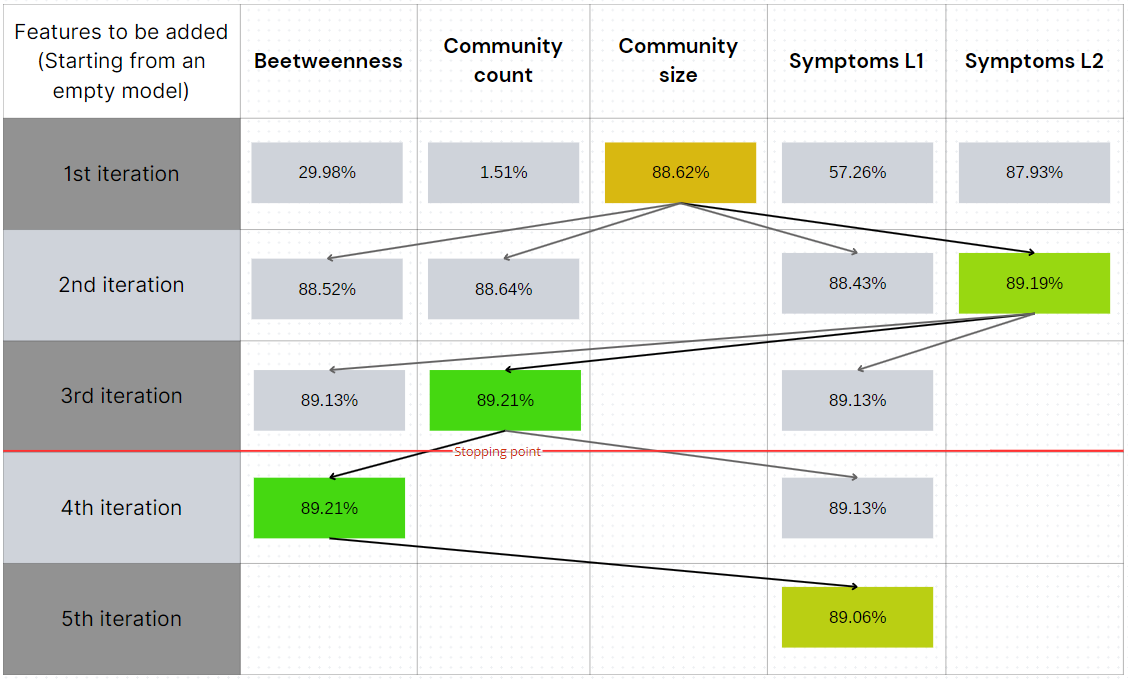
\includegraphics[width=\columnwidth]{stepwise_acc_logreg.png}
	\caption{Accuracy of the logistic regression models over the iterations of the forward stepwise feature selection}\label{fig:stepwise_acc_logreg}
\end{figure}
\noindent
Figure~\ref{fig:stepwise_acc_randomforest} shows that the random forest models behave similarly to the logistic regression,
as the best accuracy is reached after the same number of steps, employing the same features.
These results start to reveal which features are the best when it comes to classification.
It is also worth noting that the best random forest model has a slightly worse accuracy than logistic regression,
but that might be due to the random choice of the model's parameters.

\begin{figure}[H]
	\centering
	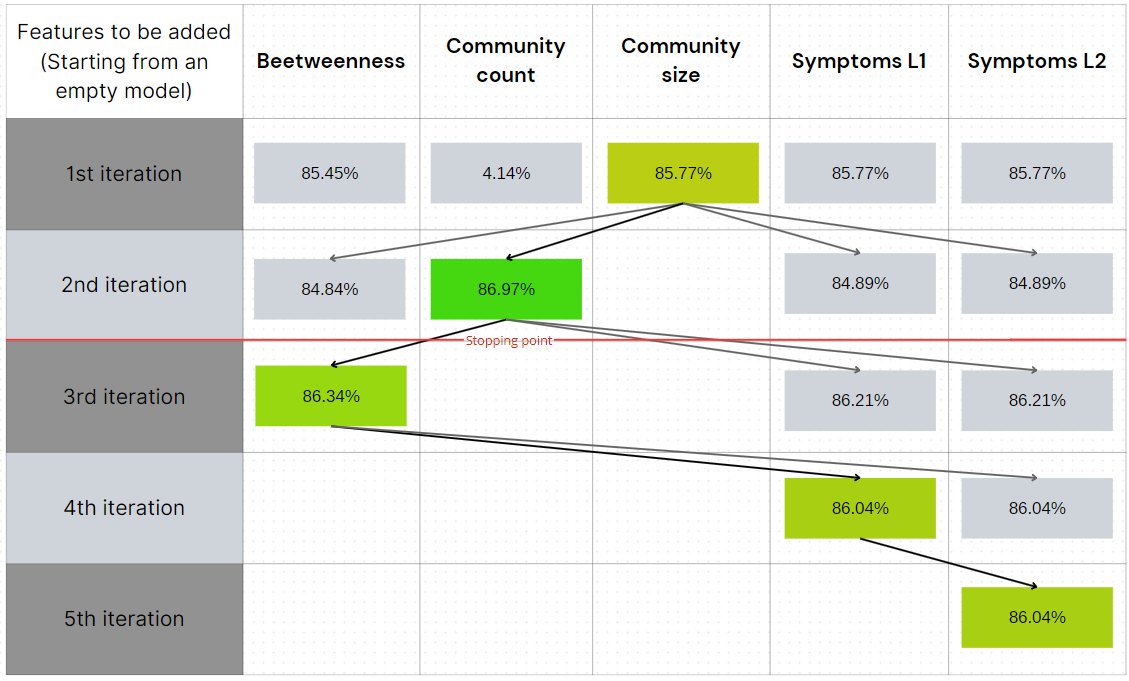
\includegraphics[width=\columnwidth]{stepwise_acc_randomforest.png}
	\caption{Accuracy of the random forest models over the iterations of the stepwise feature selection}\label{fig:stepwise_acc_randomforest}
\end{figure}
\noindent
The multi-layer perceptron model exhibits a different performance from the other two,
given by the fact that the accuracy starts to lower after adding the second feature.
As underlined by Figure~\ref{fig:stepwise_acc_mlp}, with respect to the other models information about the betweenness
is not needed to achieve the best possible results, which could be explained by the better ability of the MLP to adapt to non-linearities.
This particular implementation of neural network has one hidden layer with 100 neurons, and in our case its performance is better
than the random forest model, but still slightly worse than the logistic regression. We expect this to change after the optimization of the hyperparameters.

\begin{figure}[H]
	\centering
	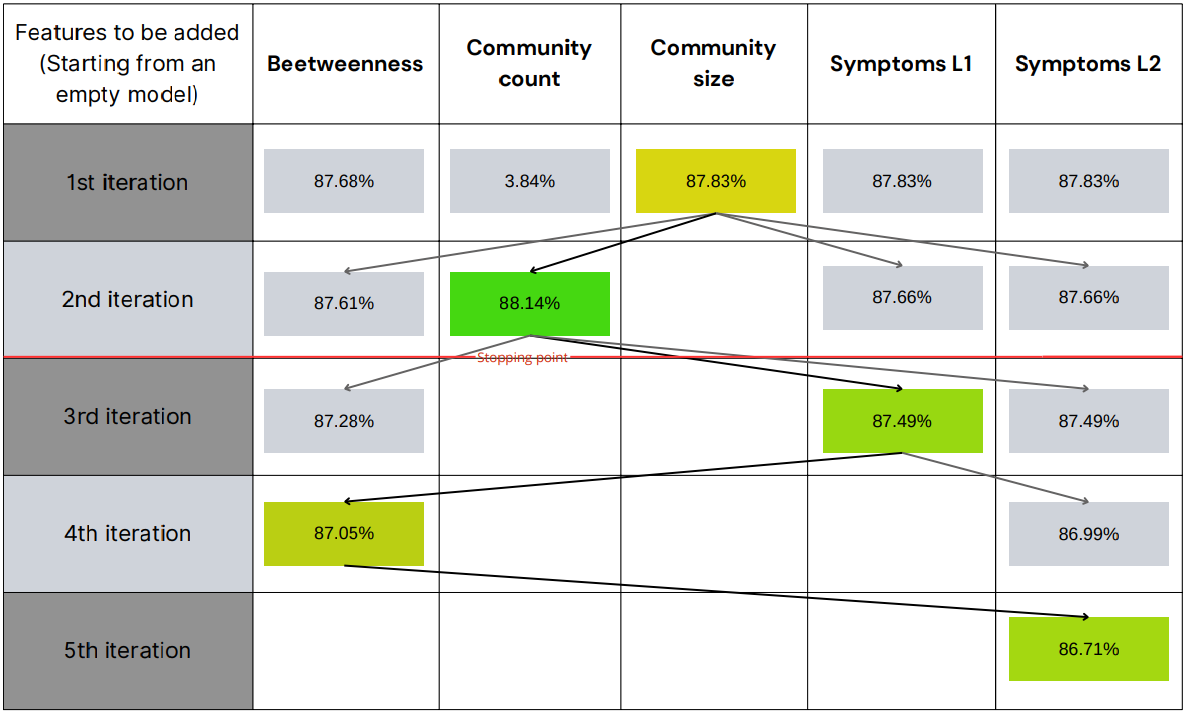
\includegraphics[width=\columnwidth]{stepwise_acc_mlp.png}
	\caption{Accuracy of the MLP models over the iterations of the stepwise feature selection}\label{fig:stepwise_acc_mlp}
\end{figure}


% CRISTIAN
% - Comparison for each model of the selected parameters --> to justify the chosen parameters
\subsubsection*{Hyperparameters Selection}


% ANDREA
% - Comparison of the three models with best combination of features and best parameters
% - precision, recall, AUC, accuracy
\subsubsection*{Model Comparison}\label{subsubsec:results_ML_model_comparison}

As illustrated in Figure~\ref{fig:ML_operative_flow}, our model ensemble now comprises six variants:
three leveraging only symptoms and three incorporating new network-based features. The selection of
the best-performing model from each group was based on test accuracy assessment, where the test is the same balanced dataset
in all cases. Figure~\ref{fig:acc_symptoms}
illustrates consistently low overfitting across all models, showcasing the stability of the symptom-only
models. In contrast, Figure~\ref{fig:acc_new_features}, portraying the accuracy of models with the new
features, reveals some overfitting, particularly in the MLP and Random Forest.\\
The observed tendency for models with new features to exhibit more pronounced overfitting is unsurprising,
given the greater number and complexity of these features compared to symptoms. Notably, despite their different
complexity, all models demonstrate similar test accuracy levels, suggesting that a linear separation
boundary suffices for effective feature classification. Considering this, we retain the Logistic Regression
model as the best-performing model in each group, striking a balance between performance and complexity.

\begin{figure}[H]
	\centering
	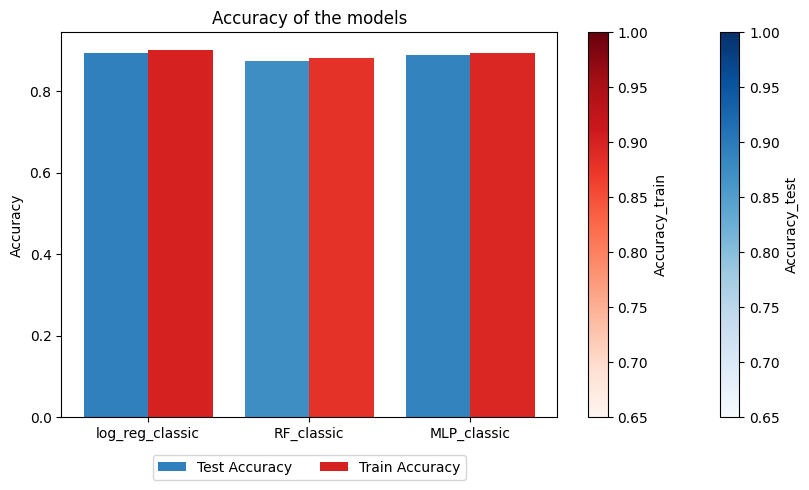
\includegraphics[width=\columnwidth]{acc_symptoms.png}
	\caption{Accuracy of the three models with only symptoms}\label{fig:acc_symptoms}
\end{figure}

\begin{figure}[H]
	\centering
	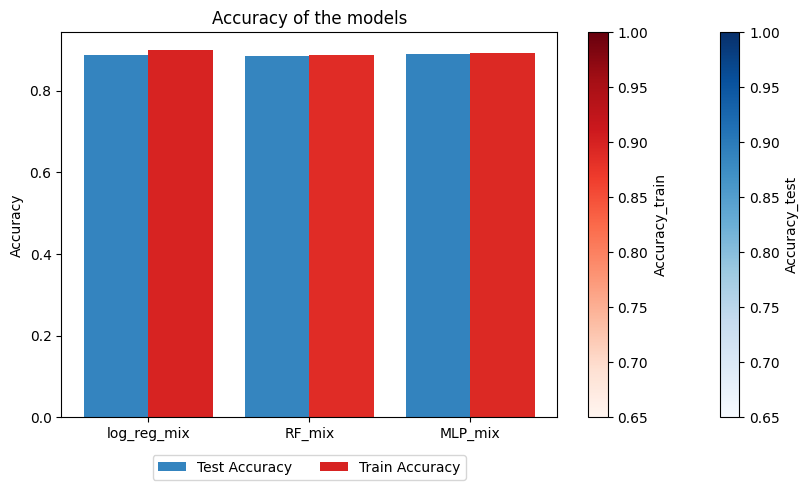
\includegraphics[width=\columnwidth]{acc_new_features.png}
	\caption{Accuracy of the three models with new features}\label{fig:acc_new_features}
\end{figure}



% --------------- New Features Effect ---------------

\subsection{New Features Effect}
% ANDREA
% - compare the best symptoms one hot model with the best one with the new features

\noindent
The best model from each group was further trained on the full balanced dataset to ensure a more reliable
performance evaluation. The results in Figure~\ref{fig:acc_best_models} reveal a minimal difference between
the two groups. This addresses our \textbf{first goal}: the new features, while not improving the model,
offer a comparable performance to using symptoms alone. However, It's essential to note that the new features are
more numerous than the symptoms, contributing to a more complex model. In conclusion, the extracted network
features are not a superior alternative to symptoms.\\
It is worth to underline that the `simplicity' of the dataset, which leads to a very high accuracy in all models, may also affect the performance
evaluation of the new features, which have a small room to improve the model. Therefore, a possible avenue
for future exploration could involve the use of more complex dataset, to better assess the performance of the
new features.\\
Another viable option for future work is to use the new features as a complement to the symptoms.


% THE FIGURE IS THE FIGURE OF MODEL FULLY TRAINED ON THE BALANCED DATASET


\begin{figure}[H]
	\centering
	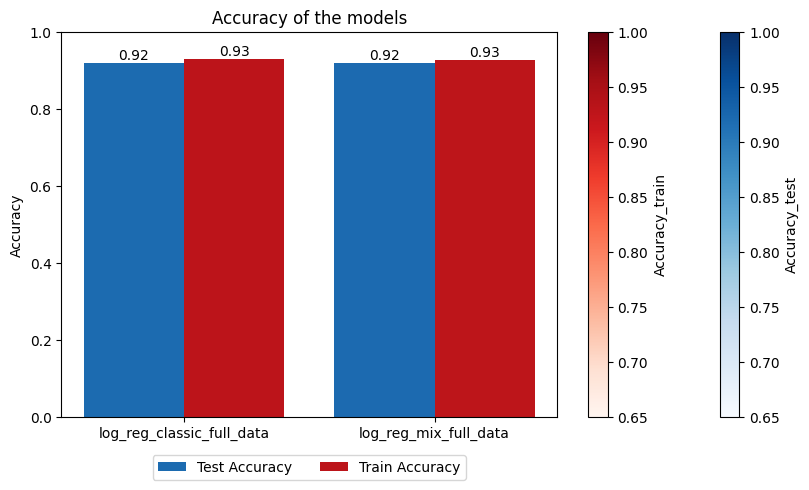
\includegraphics[width=\columnwidth]{acc_best_models.png}
	\caption{Accuracy of the best models from both groups}\label{fig:acc_best_models}
\end{figure}



% --------------- Best Model Performance ---------------

\subsection{Best Model Analysis}
Given that the logistic regression using only symptoms and the one with the new features achieve the same accuracy,
we have selected the logistic regression with the new features as the superior model for further analysis.
Considering its greater complexity and the absence of overfitting,
this model has the potential to capture more nuanced information and intricate patterns.\\
The model contains 3 group of features: community size, SI index level 2 and community count.
\subsubsection*{Performance analysis}
The performance of our predictive model, as demonstrated by the confusion matrix in Figure \ref{fig:conf_matrix},
is indicative of its capability to effectively distinguish between different disease classes.
These classes are stratified based on their respective Disease Influence (DI) indices.

\begin{itemize}
	\item \textbf{Class 1: Low DI L1 - Low DI L2:} Diseases with a low degree (DI L1) and limited connections to other symptoms (DI L2)
	      tend to be highly specific, which is reflected in the model's precision for such cases.
	      The confusion matrix exhibits a low misclassification rate for these diseases,
	      suggesting that when such specific symptoms are presented, the model can predict with high confidence,
	      albeit for a restricted number of cases.

	\item \textbf{Class 2: Low DI L1 - High DI L2:} Diseases characterized by a low DI L1 but a high DI L2 are connected to a few symptoms,
	      which in turn are associated with a wider array of other diseases. The model's performance for these diseases,
	      as shown in the confusion matrix, presents a moderate degree of accuracy.
	      Misclassifications may occur due to the broader symptom overlap with other diseases.

	\item \textbf{Class 3: High DI L1 - Low DI L2:} A high DI L1 coupled with a low DI L2 signifies diseases with numerous related symptoms,
	      which however, do not significantly influence other diseases.
	      The confusion matrix suggests that such diseases are predicted with a considerable degree of accuracy.
	      The symptoms, while not disease-specific, contribute to a heightened overall model performance due to their prevalence.

	\item \textbf{Class 4: High DI L1 - High DI L2:} Diseases with both high DI L1 and DI L2 indices are those that exhibit common symptoms
	      influencing a multitude of other diseases. The confusion matrix shows that the model is generally accurate in predicting these diseases.
	      However, due to the commonality of symptoms, there is an inherent challenge in precisely classifying them,
	      which could result in a higher misclassification rate with diseases sharing similar symptom profiles.
\end{itemize}
\noindent
The aforementioned analysis underscores the complexity inherent in disease-symptom relationships and their impact on predictive modeling.
As the confusion matrix corroborates, our model adeptly handles diseases with distinct symptom profiles (Low DI L1 - Low DI L2)
but is challenged by diseases sharing common symptoms (High DI L1 - High DI L2).
Consequently, the model's performance is a direct reflection of the nuanced interplay between disease prevalence and symptom specificity,
as encapsulated by the DI indices.
\begin{figure}[H]
	\centering
	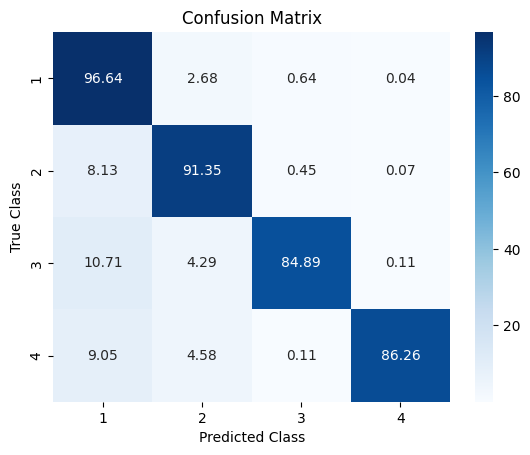
\includegraphics[width=\columnwidth]{conf_matrix_best_model.png}
	\caption{Confusion matrix of the predictive model showing the performance across the four disease classes based on DI indices.}\label{fig:conf_matrix}
\end{figure}
\noindent

\begin{figure}[H]
	\centering
	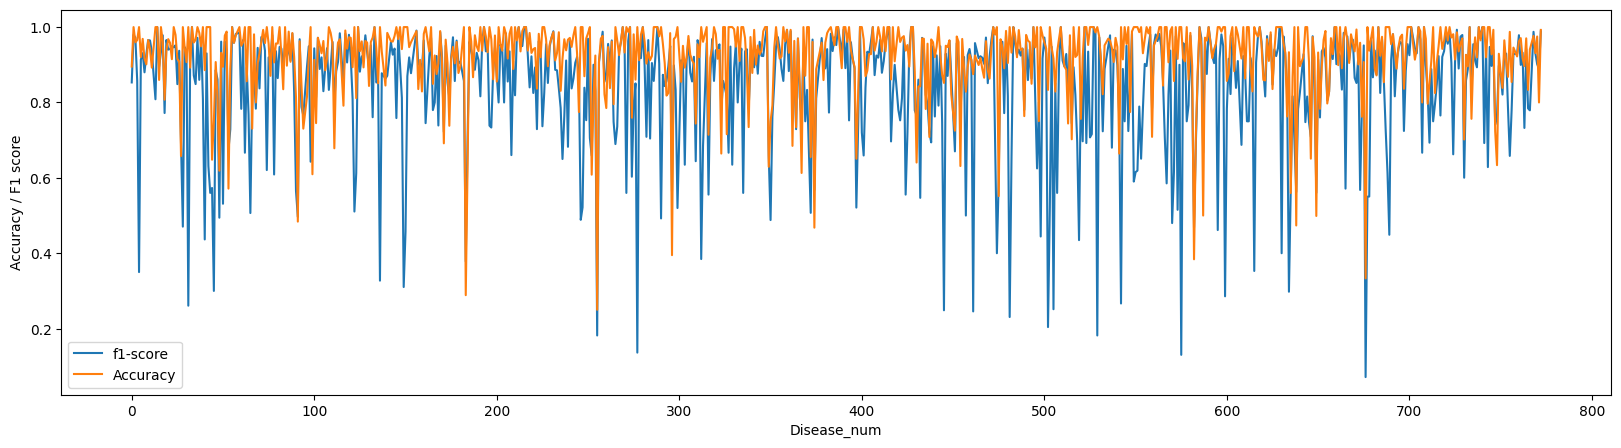
\includegraphics[width=\columnwidth]{accuraci_diseases_best_model.png}
	\caption{Accuracy and f1 score}\label{fig:acc_diseases}
\end{figure}
\noindent


\rowcolors{2}{green!8}{green!18}
\begin{table}[H]
	\centering
	\small
	\begin{tabular}{|c|c|c|}
		\hline
		\textbf{Disease}                    & \textbf{Accuracy} & \textbf{f1-score} \\
		\hline
		mitral valve disease                & 1.0               & 1.000000          \\
		syndrome of inappropriate secretion & 1.0               & 1.000000          \\
		acute bronchospasm                  & 1.0               & 1.000000          \\
		eye alignment disorder              & 1.0               & 1.000000          \\
		reactive arthritis                  & 1.0               & 1.000000          \\
		joint effusion                      & 1.0               & 0.985507          \\
		anal fistula                        & 1.0               & 0.823529          \\
		open wound of the shoulder          & 1.0               & 0.791667          \\
		alzheimer disease                   & 1.0               & 0.769231          \\
		infectious gastroenteritis          & 1.0               & 0.666667          \\
		\hline
	\end{tabular}
	\caption{Accuracy and f1 score for the 10 diseases with the highest accuracy}
	\label{best}
\end{table}


\rowcolors{2}{red!8}{red!18}
\begin{table}[H]
	\centering
	\small
	\begin{tabular}{|c|c|c|}
		\hline
		\textbf{Disease}                     & \textbf{Accuracy} & \textbf{f1-score} \\
		\hline
		premature ventricular contractions   & 0.500000          & 0.666667          \\
		histoplasmosis                       & 0.498876          & 0.560252          \\
		hemiplegia                           & 0.483908          & 0.496462          \\
		acute bronchiolitis                  & 0.473684          & 0.562500          \\
		poisoning due to antimicrobial drugs & 0.467849          & 0.567968          \\
		open wound of the mouth              & 0.394890          & 0.564315          \\
		acute otitis media                   & 0.383938          & 0.468456          \\
		vitamin b12 deficiency               & 0.333333          & 0.071429          \\
		bladder cancer                       & 0.288740          & 0.378102          \\
		otitis media                         & 0.250000          & 0.181818          \\
		\hline
	\end{tabular}
	\caption{Accuracy and f1 score for the 10 diseases with the lowest accuracy}
	\label{worst}
\end{table}

\subsubsection*{Analysis of bladder cancer}

\begin{figure}[H]
	\centering
	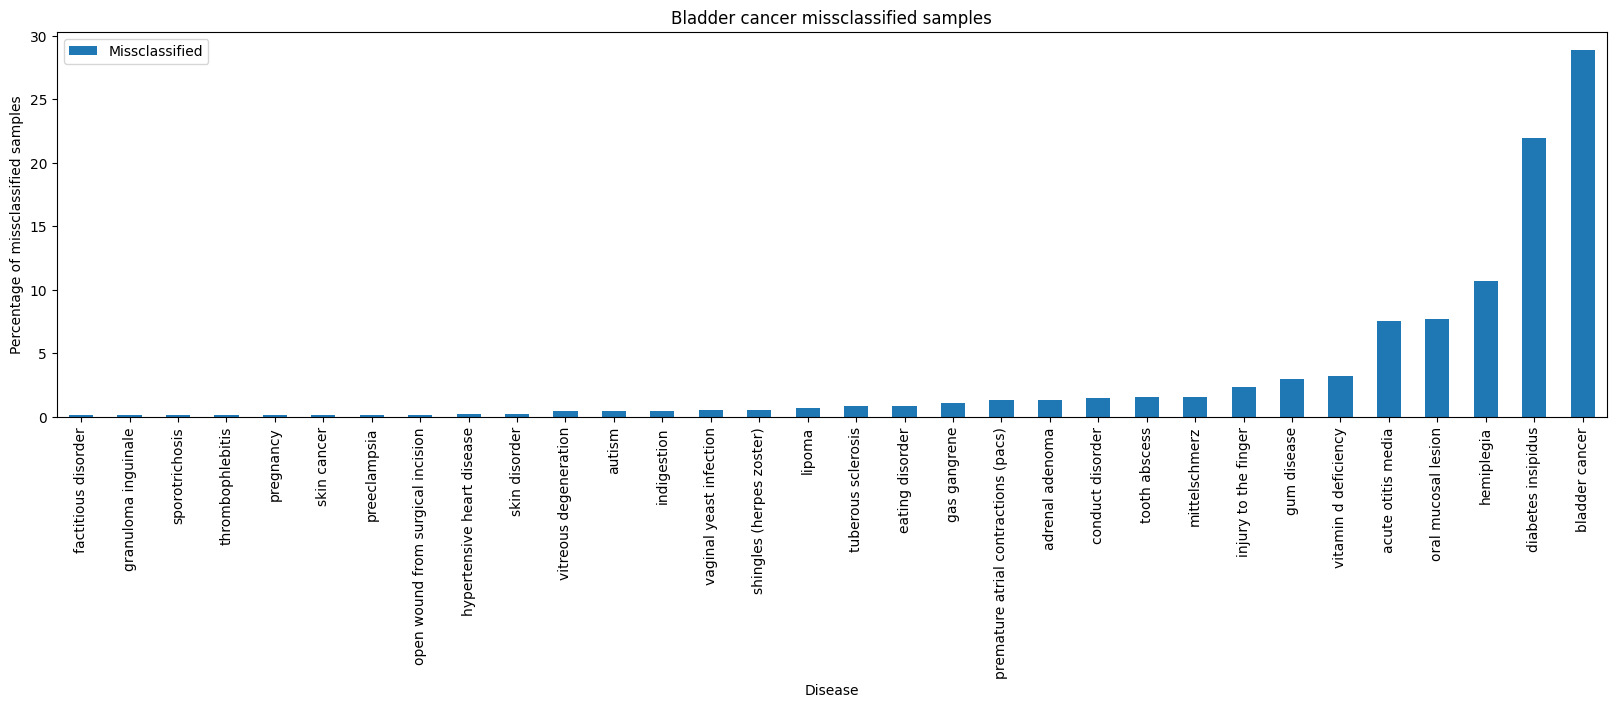
\includegraphics[width=\columnwidth]{bladder_cancer_missclassified.png}
	\caption{Percentage of bladder cancer samples misclassified}\label{fig:cancer_missclassified}
\end{figure}
\noindent

\begin{figure}[H]
	\centering
	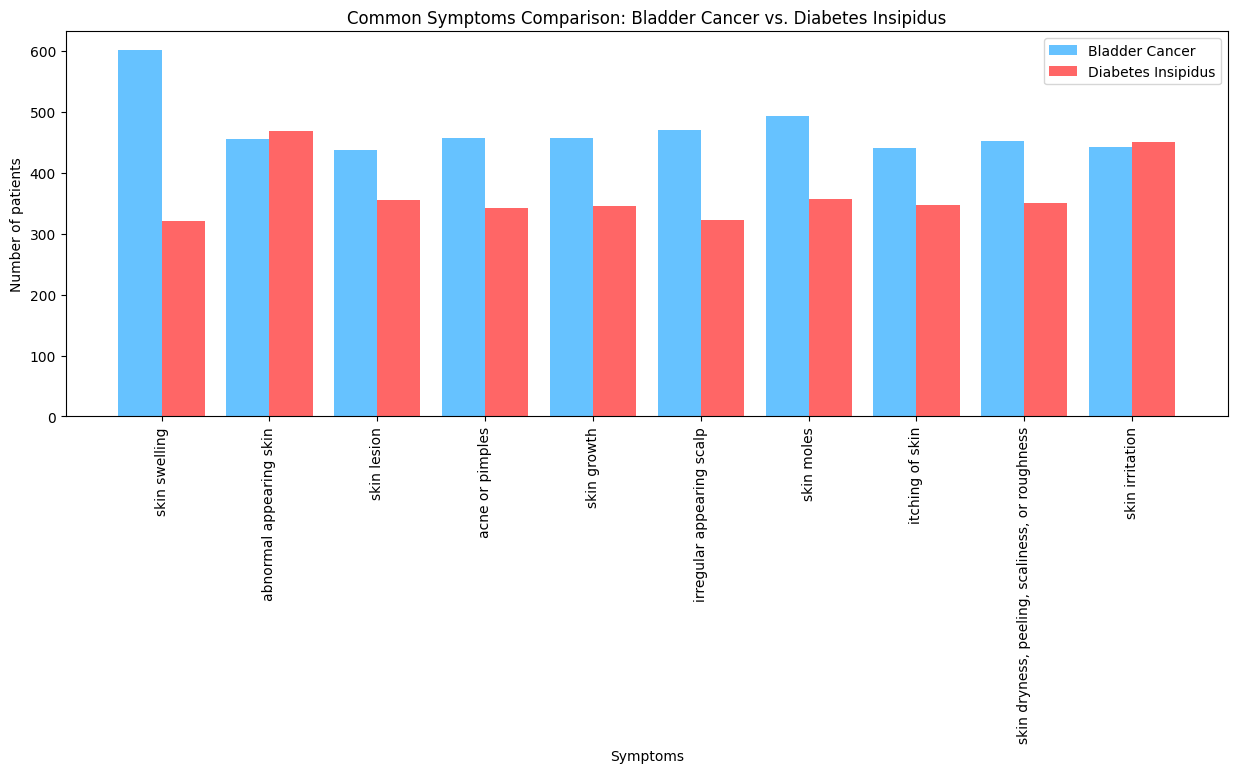
\includegraphics[width=\columnwidth]{cancer_diabet}
	\caption{number of samples of bladder cancer and diabets insipidus that have the same symptoms}\label{fig:cancer_diabet}
\end{figure}
\noindent

\begin{figure}[H]
	\centering
	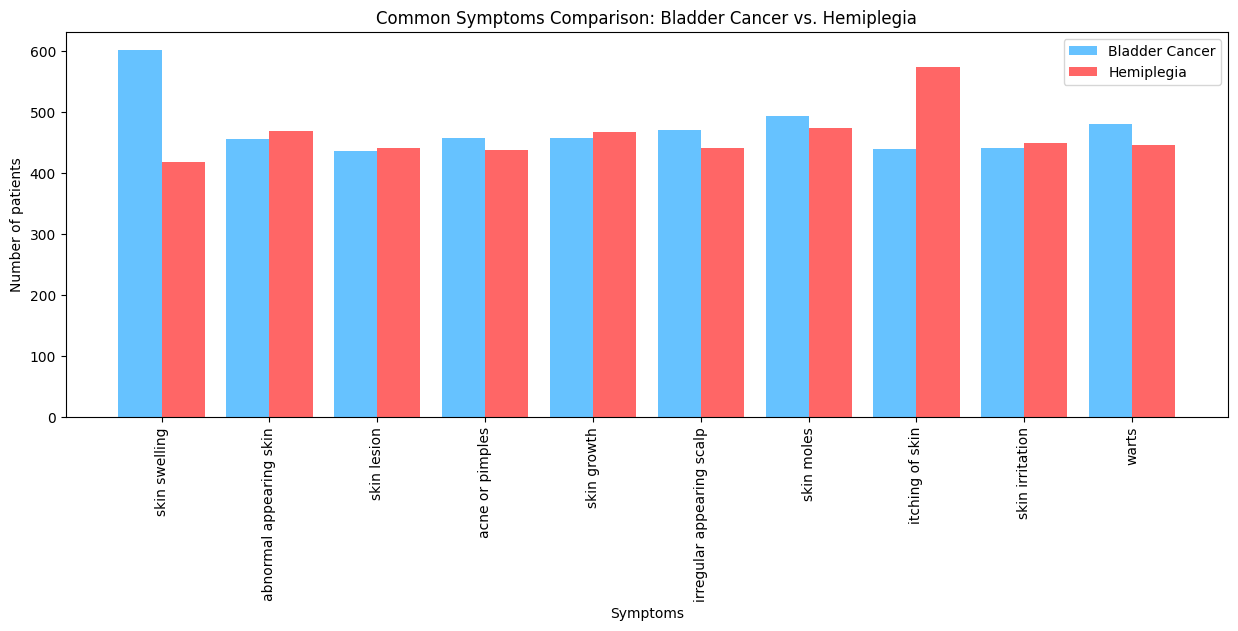
\includegraphics[width=\columnwidth]{cancer_hemiplegia.png}
	\caption{number of samples of bladder cancer and hemiplegia that have the same symptoms}\label{fig:caner_hemiplegia}
\end{figure}
\noindent

\subsubsection*{Analysis of otitis}

\begin{figure}[H]
	\centering
	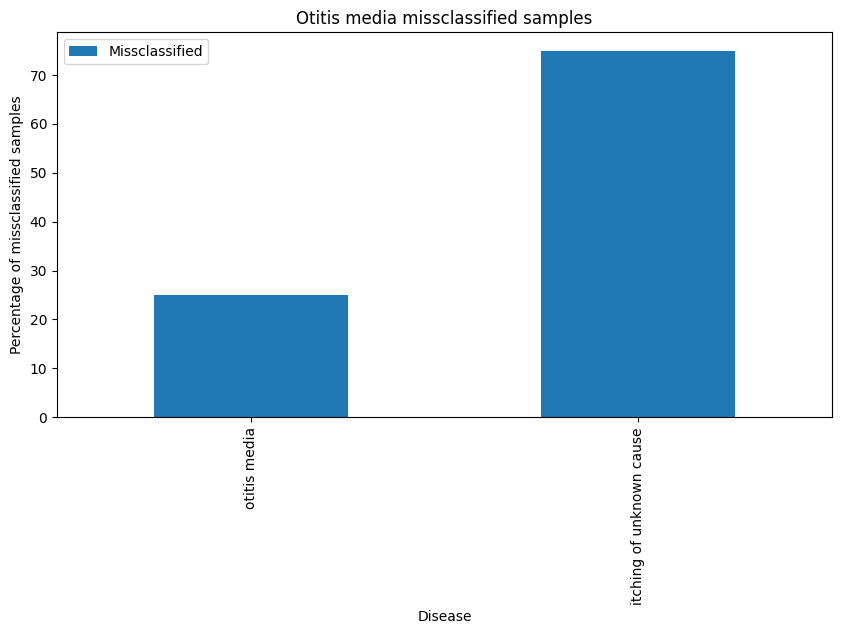
\includegraphics[width=\columnwidth]{otitis_missclassified.png}
	\caption{Percentage of otitis samples misclassified}\label{fig:otitis_missclassified}
\end{figure}
\noindent
\begin{figure}[H]
	\centering
	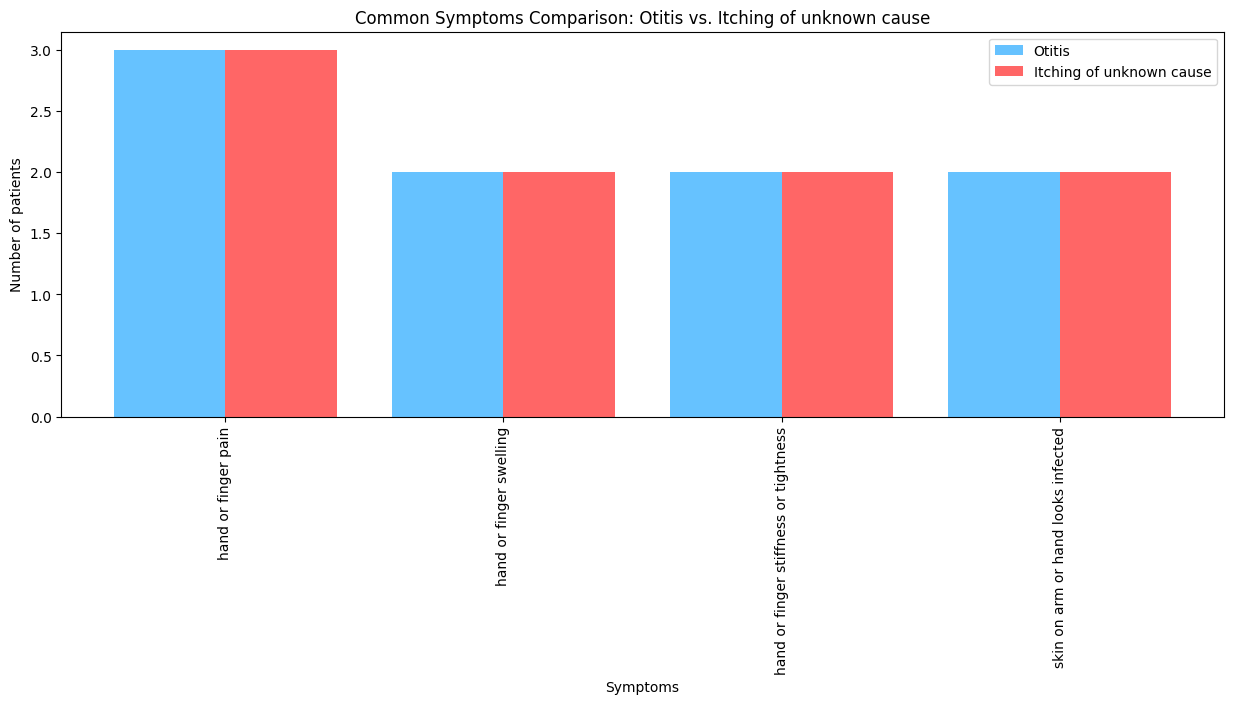
\includegraphics[width=\columnwidth]{otitis_itching.png}
	\caption{number of samples of otitis and itching of unknown cause that have the same symptoms}\label{fig:otitis_itching}
\end{figure}
\noindent

\subsection*{Most impactful symptoms}
\begin{figure}[H]
	\centering
	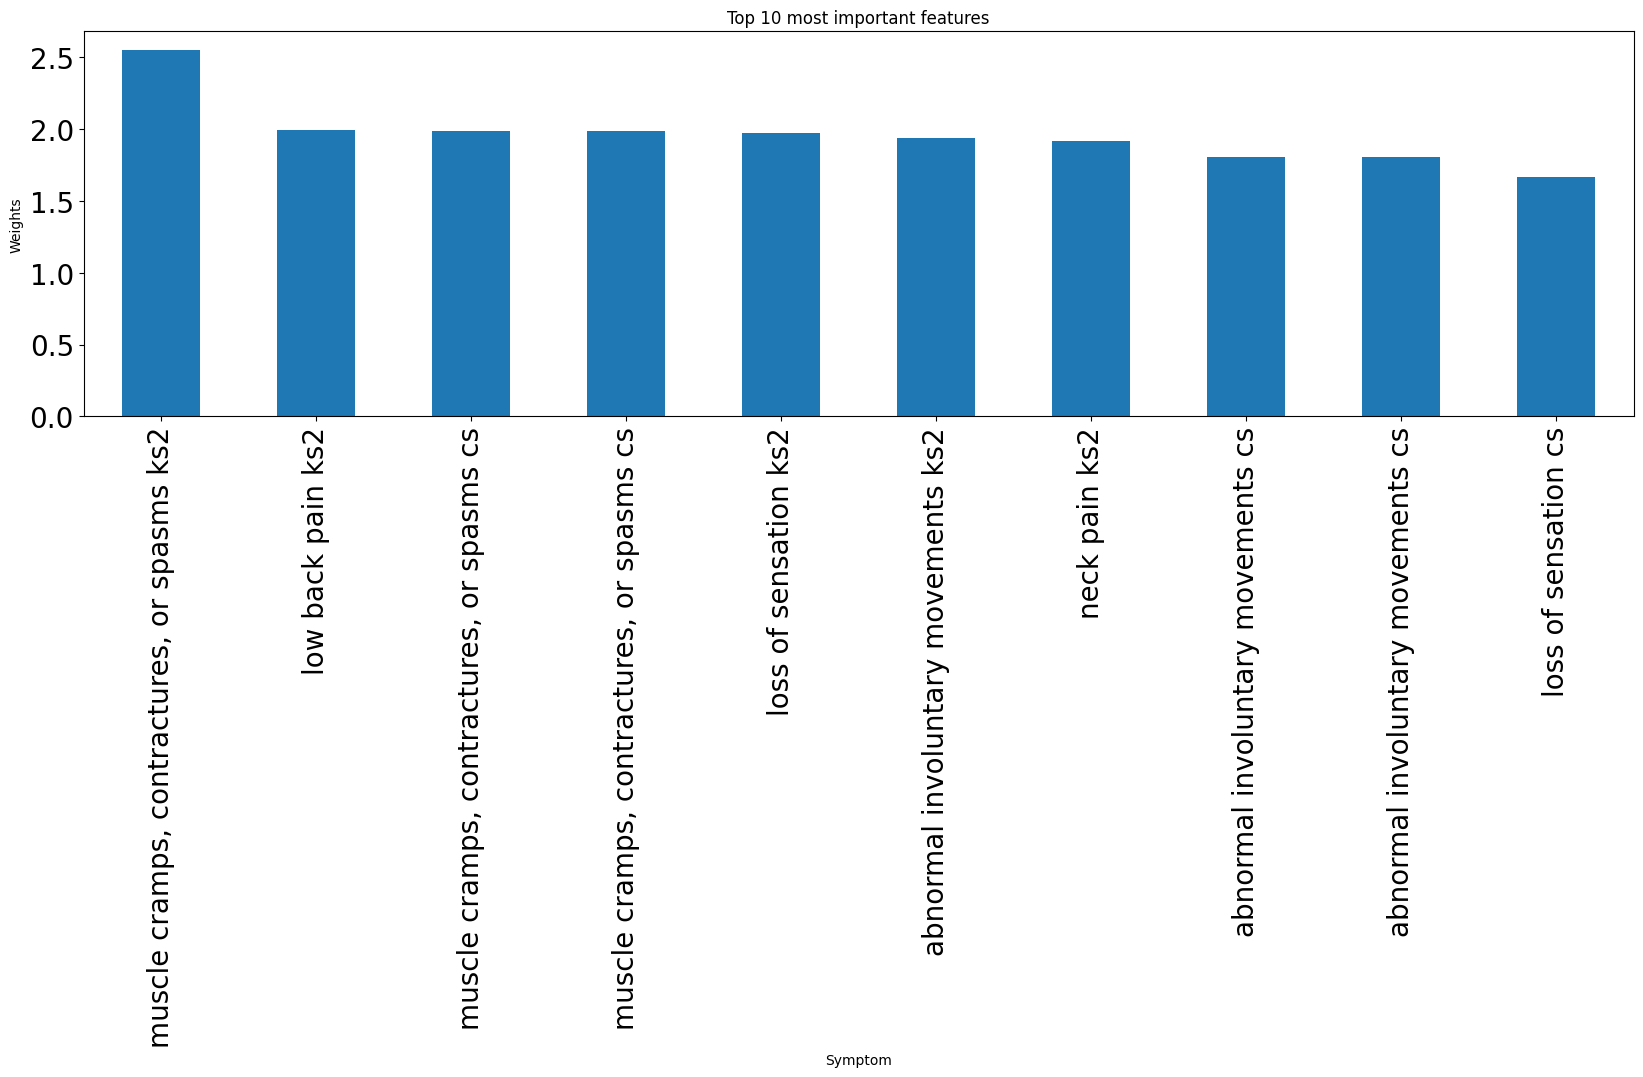
\includegraphics[width=\columnwidth]{most_important_features.png}
	\caption{10 most impactful features}\label{fig:most_important_features}
\end{figure}
\noindent

\subsection{Computational Complexity}
% MATTEO
% - apply the reduction technique based on symptoms importance (L1 and L2 combined in the 4 classes)
% - compare the performance of the reduced model with the original one
% - precision, recall, AUC, accuracy
% - compare the times needed to train the two models


% CRISTIAN
% - 6 Modelli: 3 con solo sintomi, 3 con nuove features
% - - Salvati (joblib) 
% - - Tempo di training

